\chapter{Addressing Feature Space Shortcomings through Selective Image Extraction}
\label{chapter:ch3}

This chapter will focus on the current state of Industrial Anomaly Detection, namely the use of pre-trained backbones in the unsupervised industrial anomaly detection models. We will briefly touch on the reason the pre-trained feature extractor is an irreplaceable component of contemporary models. This section will investigate the specific attributes of these models, providing insights into why they are commonly chosen for this task and how they integrate with other components of the detection system. However, we will also address potential limitations, delving into the ways in which these currently used models might actually serve as bottlenecks, hindering the overall performance and scalability of the detection systems. Further, we delve into the exploration of different feature spaces fit for the task of industrial anomaly detection. Moreover, we explore the methods by which it would be possible to generate new feature spaces that are tailor made for industrial tasks, specifically industrial anomaly detection. This will involve a detailed investigation of advanced techniques, such as selective image extraction from large-scale datasets, to create feature spaces that are more precise and capable of addressing the unique challenges presented by industrial anomaly detection.

\section{Usage of Pre-trained Feature Extractors in Contemporary Anomaly Detection Models}
\label{feature extractors}
Due to the lack of datasets with large quantity of anomalous samples and the real world use-case scenarios being the same nature, most industrial anomaly detection tasks are of the unsupervised nature. When it comes to unsupervised industrial anomaly detection, most contemporary models achieve the detection of the anomalies by performing some operations on the features extracted by pre-trained feature extractors. This approach to industrial anomaly detection was introduced by applying k-Nearest-Neighbor approach to extracted features in the paper "Deep Nearest Neighbor Anomaly Detection". Due to the efficacy of k-Nearest-Neighbor in general anomaly detection tasks, including anomaly detection on tabular data, it has been proposed that the approach would work for anomaly detection in image data. The paper compares performing kNN on raw images against kNN on extracted features from a pre-trained feature extractor, showing that the latter method shows promising performance. Since, unsupervised industrial anomaly detection models use methods such as kNN, clusterization, auto-encoders etc. on extracted features to achieve high accuracy anomaly detection. By leveraging pre-trained feature extractors, these models can bypass the need for extensive labeled datasets, which are often scarce in industrial settings, thus benefiting from the vast amounts of data and learning already captured in these pre-trained models, thereby enhancing their detection capability.

\begin{figure}[t]
	\begin{center}
		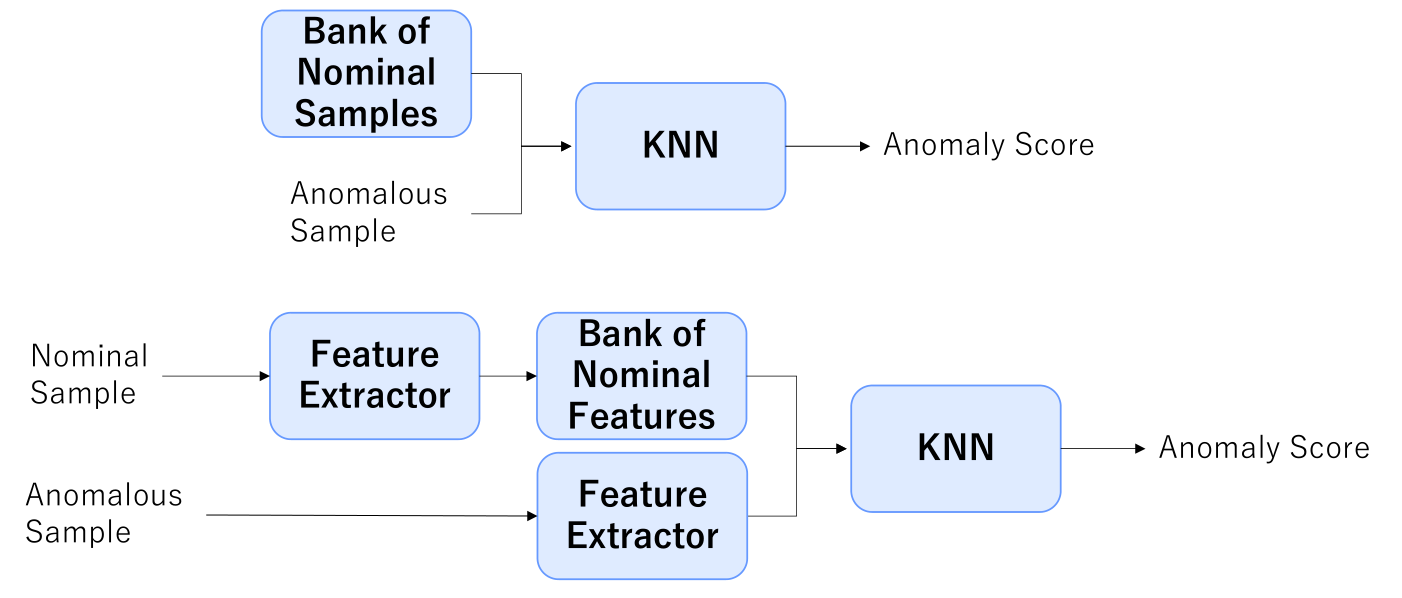
\includegraphics[width=1.0\linewidth]{Chapter_3/feature_extractor_usage.png}
	\end{center}
	\caption{Convolutional Neural Network consisting of convolution and subsampling layers. Its architecture allows for the efficient capture of spatial features, which can explain its prominence in anomaly detection models.}
	\label{fig:cnn}
\end{figure} 	

\section{Commonly Used Pre-trained Extractors}
\label{common extractors}
As will be demonstrated by the experiments further in the Chapter~\ref{chapter:ch4} the most commonly used type of models as feature extractors in the industrial anomaly detection models are the convolutional models, specifically residual networks. The case is that residual networks significantly outperform vision transformers as feature extractors for anomaly detection models. This occurrence might be explained by the fact that convolutional models have the higher capacity to capture spatial hierarchies and local relationships than the vision transformer architectures. Throughout all the state-of-the-art industrial anomaly detection models, the common practice is to use feature extractors pre-trained on ImageNet dataset on a supervised classification task. This pre-training on ImageNet allows the models to leverage a vast amount of general knowledge, which can then be fine-tuned to the specific requirements of industrial anomaly detection. ImageNet pre-trained feature extractor are common in all the fields of machine learning including industrial anomaly detection due to the extensiveness and generality of ImageNet dataset. This thesis will further explore these aspects through detailed experiments and analyses, providing a comprehensive understanding of why ResNets remain the backbone of state-of-the-art industrial anomaly detection models.

\subsection{Potential Drawbacks of ImageNet Pre-trained Feature Extractors}
\label{imagenet pre-trained}
The use of ImageNet pre-trained feature extractors could carry some hidden potential drawbacks when used in industrial anomaly detection. ImageNet dataset consists of wide variety of categories, including manufactured objects alongside with natural samples, humans etc. This diverse nature is indeed beneficial for many general-purpose applications, as it allows for robust feature learning across many domains. Meanwhile, most industrial anomaly detection datasets consist of close up shots of manufactured objects like screws, pills, transistors etc, which require a different focus and precision. As we can observe, the nature of samples found in ImageNet dataset have a discrepancy from the samples that would be found in usual industrial anomaly detection task. Features learned from general purpose datasets such as ImageNet could match industrial features with less accuracy than a feature learned from a specialized dataset. Therefore, it raises the question of whether the apparent convenience of using such well-established models truly outweighs the potential benefits of training models on more specialized datasets tailored to specific industrial needs.

\begin{figure}[t]
	\begin{center}
		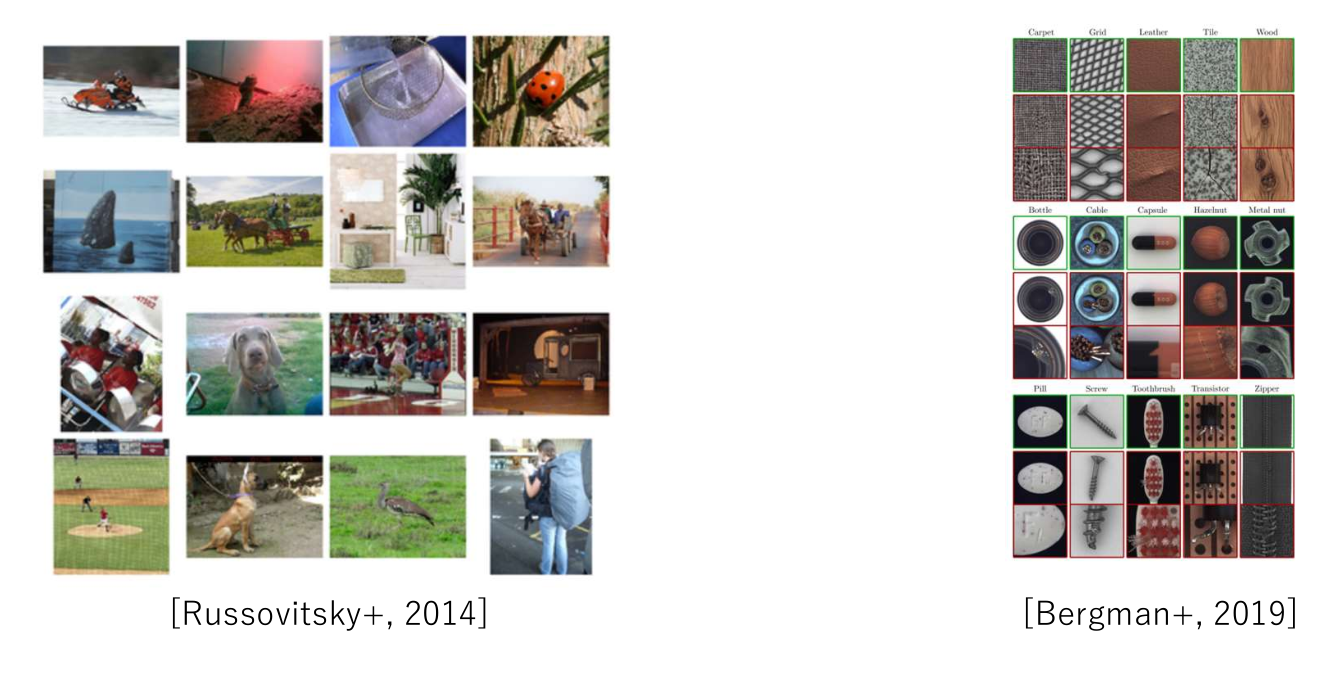
\includegraphics[width=1.0\linewidth]{Chapter_3/discrepancy.png}
	\end{center}
	\caption{Convolutional Neural Network consisting of convolution and subsampling layers. Its architecture allows for the efficient capture of spatial features, which can explain its prominence in anomaly detection models.}
	\label{fig:cnn}
\end{figure} 	

\section{Addressing the Drawbacks Through Exploration of Various Feature Spaces}
\label{addressing the drawbacks}
To test the hypothesis stated above, in this thesis, we decided to test the performance of multiple pre-trained feature extractors on the against each other on the same industrial anomaly detection models. Firstly, we want to find out which architectures would learn the most effective features from the datasets we are going to construct in the future steps. Our goal is not only to identify the most suitable architecture but also to gain insight into how different architectures handle industrial data, especially given the unique challenges presented by these datasets. In order to determine the best architecture we test multiple ImageNet pre-trained models with different architectures on the identical industrial anomaly detection model. Further, after the result of this analysis on model architecture, we move on to the exploration of methods for generation of suitable feature spaces.

\section{Construction of Industrial Anomaly Detection Specialized Feature Spaces}
\label{construction}
There are multiple approaches to constructing the possibly suitable feature spaces for industrial tasks. These approaches can be separated mainly into two types: methods that involve enhancing or modifying the feature spaces extracted from ImageNet dataset, methods that consist of assembling a dataset that would be closely related to industrial setting. An example for the first method would be introducing random or synthetic noise to the randomly selected features learned from ImageNet. In this thesis, however, we mainly focus on, and propose multiple ways to accomplish feature space generation by the second method. First approach we explore is the extracting industrial subset from the large scale, general purpose dataset using a CNN classifier as an extractor and learning feature form that subset. Second approach is similar to the first one, with the exception that, instead of using a CNN classifier, we utilize the combination of an LLM and a VLM.

\begin{figure}[t]
	\begin{center}
		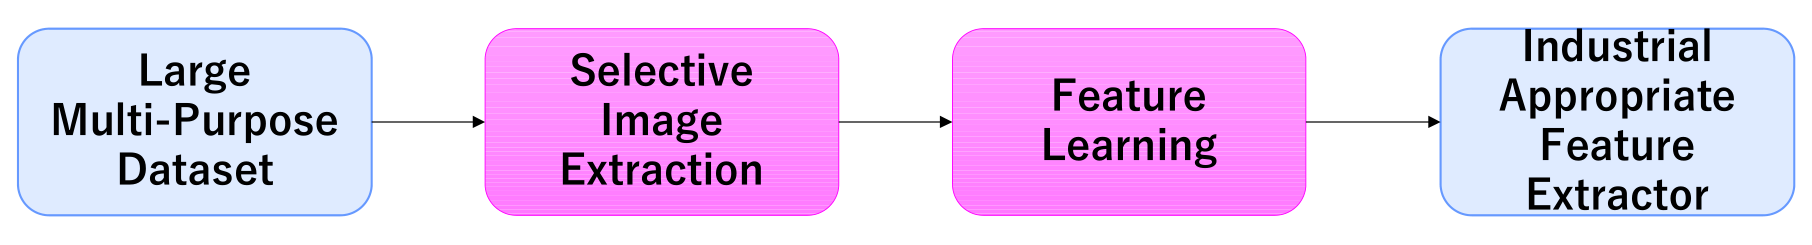
\includegraphics[width=1.0\linewidth]{Chapter_3/selective_extraction.png}
	\end{center}
	\caption{Convolutional Neural Network consisting of convolution and subsampling layers. Its architecture allows for the efficient capture of spatial features, which can explain its prominence in anomaly detection models.}
	\label{fig:cnn}
\end{figure} 	

\section{Selective Extraction With Bi-Class CNN Classifier}
\label{cnn extraction}
As mentioned before, first approach we will be discussing thoroughly is utilizing a bi-class CNN classifier to extract a industrial setting specific subset from the a large scale multi purpose dataset. The process consists of two stages, which are training the bi-class CNN classifier and selecting for industrial images using the trained model. The bi-class classifier will be trained to sort images into two classes: industrial and non-industrial. Once the training phase is complete, the classifier will be utilized to filter through the extensive dataset, flagging and selecting images that fall under the industrial category. Our goal is to achieve precise extraction of industrial setting images, from which, further learning of useful industrial specialized features can be achieved. 

\subsection{Assembling the Bi-Class Classifier}
\label{bi-class assemble}
The procedure of training the bi-class CNN classifier is a standard classification task training on the dataset that consists of samples of two classes, which are "industrial" and "non-industrial". Firstly, we are required a dataset with such classes, which will be acquired by manually splitting labeled multi-purpose dataset. In the case of this thesis, due to its versatility and large scale, the decision has been made to choose the dataset ImageNet. Further, we split the images in the ImageNet dataset by 1000 classes, having 454 industrial classes and 546 non-industrial classes. Finally, in order to achieve a trained CNN classifier model in a more robust way, we can leverage an ImageNet pre-trained model due to the fact that the new built dataset mostly consist of samples from ImageNet dataset.

\begin{figure}[t]
	\begin{center}
		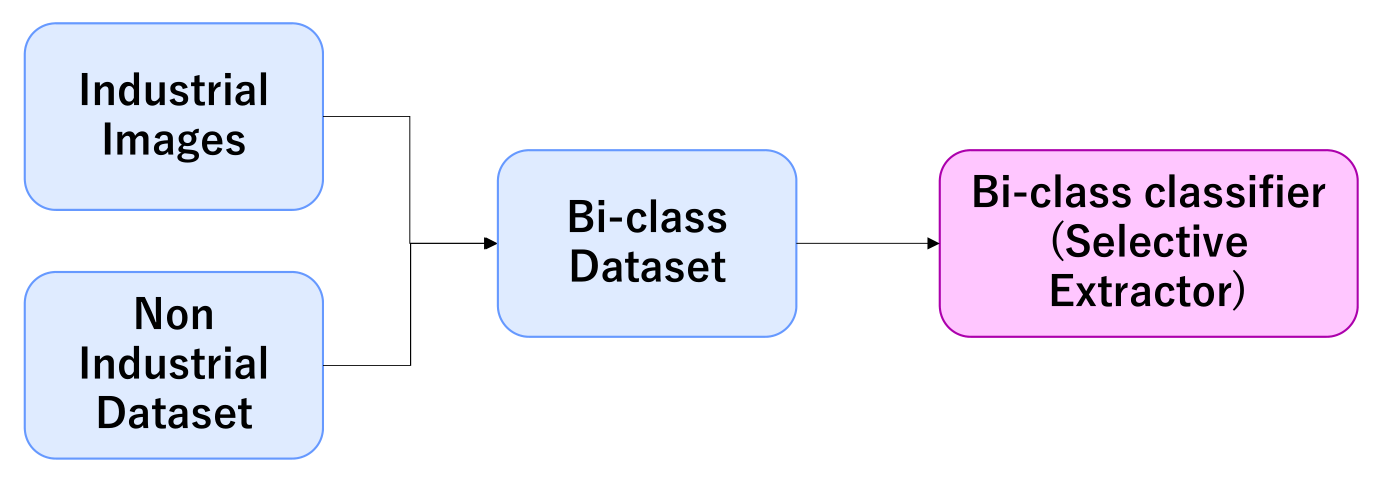
\includegraphics[width=1.0\linewidth]{Chapter_3/cnn_train_data.png}
	\end{center}
	\caption{Convolutional Neural Network consisting of convolution and subsampling layers. Its architecture allows for the efficient capture of spatial features, which can explain its prominence in anomaly detection models.}
	\label{fig:cnn}
\end{figure} 	

The extraction process will be discussed in the next section more thoroughly, however, before moving on to it, an important point should be brought to attention. The point is, after the first selection attempts, through manual visual analysis of the extracted samples, it has been revealed that the extractor model shows bias towards human faces for the "industrial" class. To alleviate this issue, two measures are taken: inclusion of the samples from "Labeled Faces in Wild" into the "non-industrial" subset and extraction of images with prominently shown faces in them using "YOLOv5" object detection. After performing listed actions, the performance of the selective extractor appeared to be acceptable according to manual visual analysis.

\subsection{Selective Extraction}
\label{cnn selective extraction}
Utilizing the CNN selective image extractor, the database for feature learning can be formed. The construction of dataset is performed by classifying images in a large multi-purpose dataset, which is in the case of this work will be the YFCC100M dataset. The choice of this particular dataset is motivated by the necessity of easily accessible and versatile dataset. By performing the classification, the bi-class CNN classifier can effectively sift through the vast YFCC100M dataset, isolating and extracting a subset of images that are assumed to be related to industrial settings. Furthermore, upon visual inspection of the extracted samples, it becomes evident that there is a noticeable bias towards industrial images, indicating the efficacy of the bi-class CNN classifier in accurately identifying and selecting industrial-relevant samples.

\subsection{Feature Learning}
\label{feature learning cnn}
Due to the nature of the selective extraction method, the resultant dataset comprises solely of the "industrial" class for all the samples extracted. Given that supervised classification task training necessitates the presence of multiple classes within a dataset, utilizing this single-class dataset for such tasks is evidently not feasible. To circumvent this limitation, we opt for an unsupervised learning approach. Specifically, we employ a self-supervised learning model known as DINO to extract meaningful features from the vast, unlabeled dataset of industrial images. For a more in-depth discussion of the DINO model and its underlying mechanisms, readers are referred to Chapter~\ref{chapter:ch2}, where detailed explanations and examples are provided.

\begin{figure}[t]
	\begin{center}
		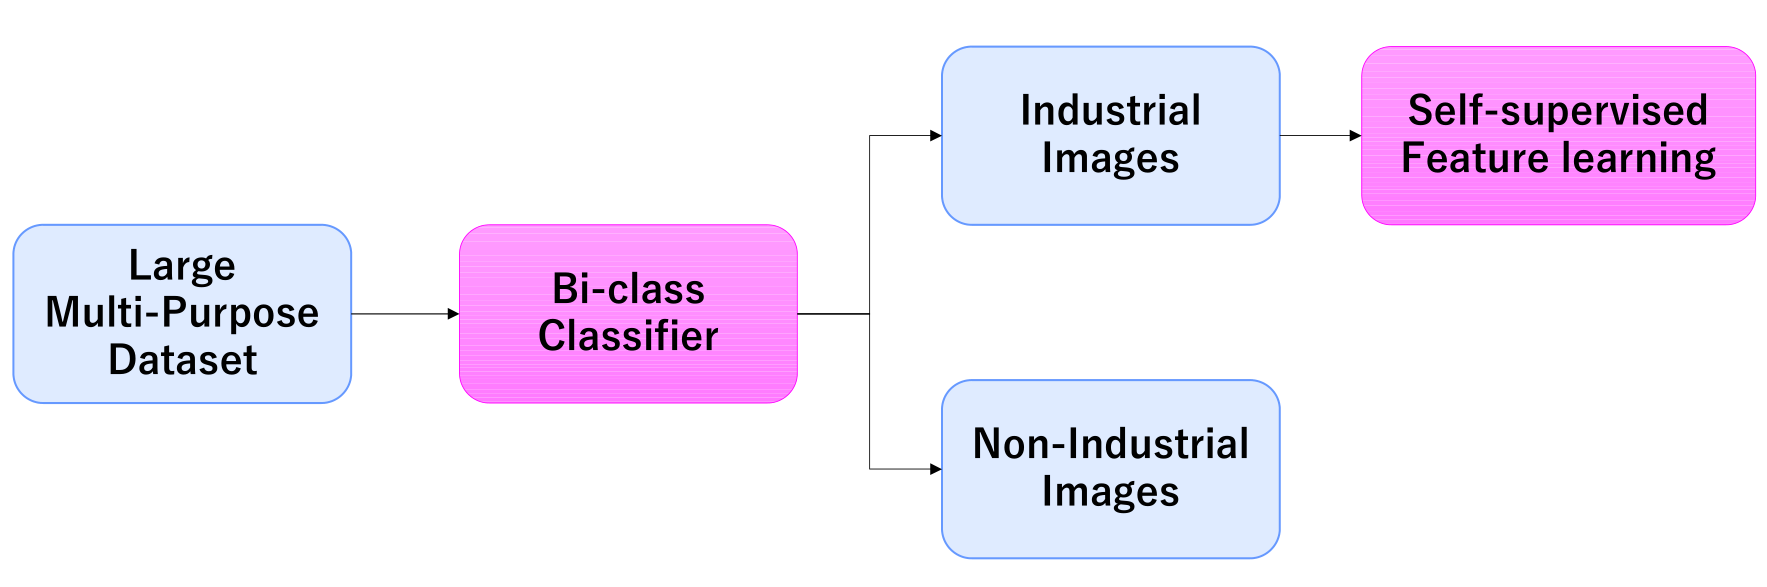
\includegraphics[width=1.0\linewidth]{Chapter_3/cnn_extraction.png}
	\end{center}
	\caption{Convolutional Neural Network consisting of convolution and subsampling layers. Its architecture allows for the efficient capture of spatial features, which can explain its prominence in anomaly detection models.}
	\label{fig:cnn}
\end{figure} 	

\section{Selective Extraction With an LLM and a VLM}
\label{llm and vlm extraction}
The second approach to the selective extraction that is proposed in this thesis is the utilization of the combination of an LLM(Large Language Model) and an VLM(Vision Language Model). The pipeline of the selective extraction by this method consists of two major stages, which are generation of descriptions using an LLM and filtration by a cosine similarity threshold with the help of an VLM. For this work we chose GPT-3 model as the LLM and CLIP model as the VLM. This method can function in specialized manner and in a general manner. When used in a specialized manner, it is possible to generate descriptions that would select for images that are close in feature to a specific use case. In generalized style of functioning, we generate descriptions that are related to the word "industrial", "manufacturing" etc. In the case of this thesis, we focus on improving the performance on the dataset MVTechAD in order to test the efficiency of the method in constrained boundaries. The steps to utilize the method with focus on MVTechAD are as follows: using specific prompts to generate descriptions and extracting images using the CLIP model.

The first prompt to the GPT-3 model is as follows:

"give a python array containing the word "transistor" and it's synonyms, include as much synonyms as possible but avoid unrelated words"

afterwards, the following prompt is given:

"generate description for use in a CLIP model using these generated words, each word should be used in at least one description. One description should contain at least one word from the list. Generate as much descriptions as possible. Output as python array"

This process generates description for a single category in the MVTechAD dataset. Further, the same procedure is applied to the remaining categories in the dataset.

To determine the threshold value that is used for the extraction process, we apply CLIP with the descriptions specific to a category in the MVTechAD dataset to the images in the same category. Through the aforementioned approach the value of 0.29 was determined to be optimal to extract images. Every image that passes the threshold 0.29 on any of the descriptions are selected from the YFCC100M dataset. 

\begin{figure}[t]
	\begin{center}
		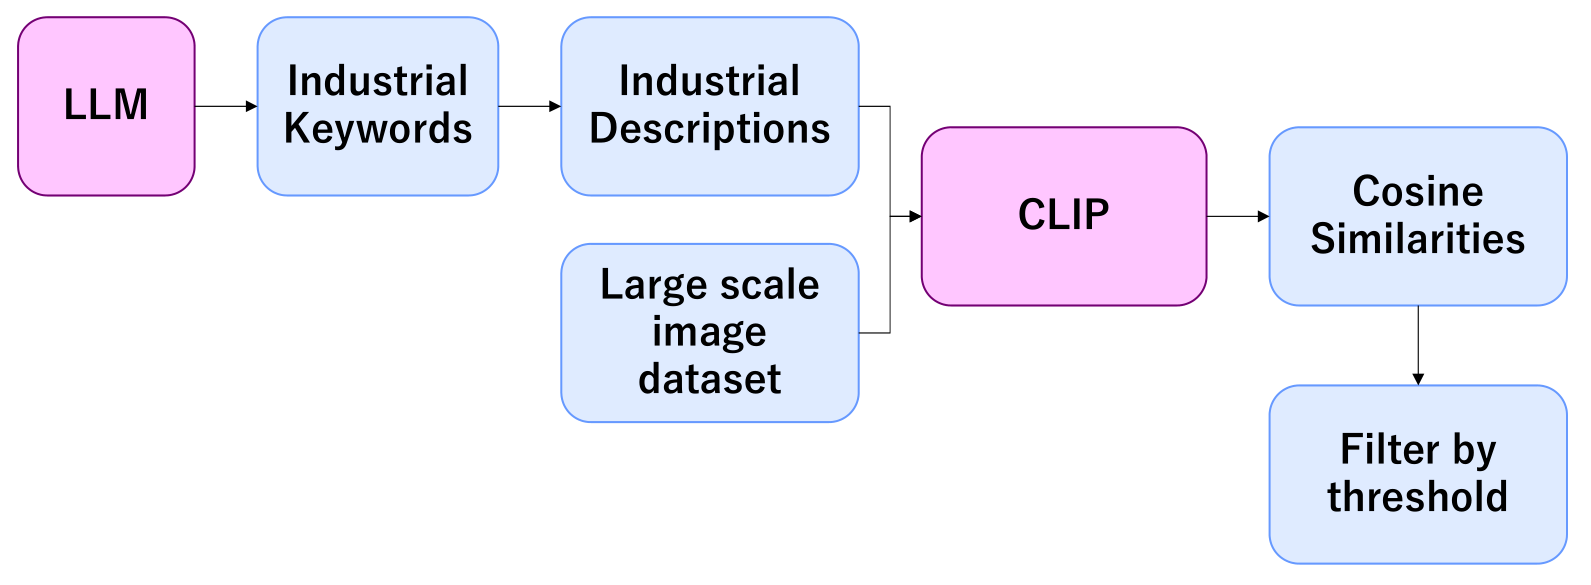
\includegraphics[width=1.0\linewidth]{Chapter_3/llm_extraction.png}
	\end{center}
	\caption{Convolutional Neural Network consisting of convolution and subsampling layers. Its architecture allows for the efficient capture of spatial features, which can explain its prominence in anomaly detection models.}
	\label{fig:cnn}
\end{figure} 	

\subsection{Feature Learning}
\label{feature learning llm}
The use of base keywords, which are in this case categories from MVTechAD dataset, makes it possible to assemble a labeled dataset, unlike the method with the bi-class CNN classifier. This property of the method of extraction creates a possibility of feature learning through supervised classification task training. Supervised learning is accomplished by using the base keywords that are given in the former prompts, which are, in the of this thesis, the categories in the dataset MVTechAD. Moreover, we use the features of the ImageNet pre-trained model as the starting point and perform a fine-tuning instead of learning features from scratch. The performance of ImageNet features on the industrial anomaly detection makes them a good starting point for training.

\begin{figure}[t]
	\begin{center}
		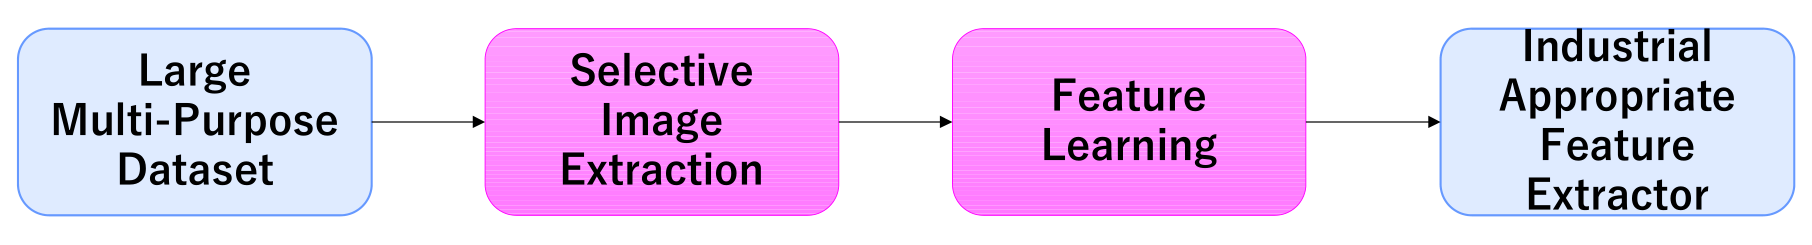
\includegraphics[width=1.0\linewidth]{Chapter_3/selective_extraction.png}
	\end{center}
	\caption{Convolutional Neural Network consisting of convolution and subsampling layers. Its architecture allows for the efficient capture of spatial features, which can explain its prominence in anomaly detection models.}
	\label{fig:cnn}
\end{figure} 	
